
\subsection{Statement}

This section deals with the steady state version of the problem proposed by Smith and Hutton (1982). The problem takes place in the domain $\Omega = (-L,L) \times (0,L) \subset \real$ where $L > 0$ is a constant. In it the steady state version of the general convection--diffusion equation is considered
\begin{equation}
	\rho \vb{v} \vdot \grad{\phi} = \div(\Gamma \grad{\phi}) + \dot{s}_\phi
\end{equation}
On the boundary of $\Omega$ the following conditions are prescribed:
\begin{itemize}[topsep=0pt]
	\item $\phi = 1 + \tanh(10(2x+1))$ on $[-L,0] \times \{ y = 0 \}$ (inlet flow).
	\item $\frac{\partial \phi}{\partial y} = 0$ on $(0,L] \times \{ y = 0 \}$ (outlet flow).
	\item $\phi = 1 - \tanh(10)$ on $(\partial \Omega) \setminus ([-L,L] \times \{ y = 0 \})$. 
\end{itemize}
The velocity field is given by $v_x = 2 y (1 - x^2)$ and $v_y = -2 x (1 - y^2)$, which verifies the incompressibility condition since $\div{\vb{v}} = 0$.

\begin{figure}[h]
	\centering
	\begin{tikzpicture}
		% Lenghts
		\def\alength{5}
		\def\L{4.5}
		\def\mlength{0.1}
		% Domain
		\fill[cyan!70!white] (-\L,0) rectangle (\L, \L);
		\draw[thick, thick] (-\L,0) rectangle (\L, \L);
		% Axis
		\draw[-stealth] (-\alength,0) -- (\alength,0) node[above]{$x$};
		\draw[-stealth] (0,-0.5) -- (0,\alength) node[right]{$y$};
		\draw[black, thick] (\L,0) -- ++(0,-\mlength) node[below]{$L$};
		\draw[black, thick] (-\L,0) -- ++(0,-\mlength) node[below]{$-L$};
		\draw[black, thick] (0,\L) -- ++(-\mlength,0) node[left, yshift=2mm]{$L$};
		% Right boundary condition
		\node[inner sep=0pt] at (\L,{0.5*\L}) (rb) {};
		\node[] at ({\L+2},{0.5*\L+1}) (rbc) {$\phi = 1 - \tanh(10)$};
		\path[-latex] (rbc) edge[bend left] node [left] {} (rb);
		% Top boundary condition
		\node[inner sep=0pt] at ({0.1*\L},\L) (tb) {};
		\node[] at ({0.1*\L+2},{\L+1}) (tbc) {$\phi = 1 - \tanh(10)$};
		\path[-latex] (tbc) edge[bend right] node [left] {} (tb);
		% Left boundary condition
		\node[inner sep=0pt] at (-\L,{0.5*\L}) (lb) {};
		\node[] at (-\L-2,{0.5*\L-1}) (lbc) {$\phi = 1 - \tanh(10)$};
		\path[-latex] (lbc) edge[bend left] node [left] {} (lb);
		% Right bottom boundary condition
		\node[inner sep=0pt] at ({0.5*\L},0) (bb) {};
		\node[] at ({0.5*\L-1},-1) (bbc) {$\dfrac{\partial \phi}{\partial y} = 0$};
		\path[-latex] (bbc) edge[bend right] node [left] {} (bb);
		% Left bottom boundary condition
		\node[inner sep=0pt] at ({-0.5*\L},0) (lbb) {};
		\node[] at ({-0.5*\L-1},-1) (lbbc) {$\phi = 1 + \tanh(10(2x+1))$};
		\path[-latex] (lbbc) edge[bend right] node [left] {} (lbb);
		% PDE outer sep=0pt, greenNode, yshift=3mm, fill=white
		\node[fill=cyan!70!white] at (0,{0.5*\L}) 
		{$\Delta{\phi} - \beta \left( \pdv{\phi}{x} + \pdv{\phi}{x} \right) = 0$};
		% Inlet and outlet
		\node[] at ({-0.5*\L},0.3) {Inlet};
		\node[] at ({0.5*\L},0.3) {Outlet};
	\end{tikzpicture}
	\caption{Cauchy problem for the diagonal flow case.}
	\label{fig:case_diagonal_flow_statement}
\end{figure}


